\documentclass[11pt]{article}
\usepackage[pdftex]{graphicx}
\usepackage{amsmath}
 \usepackage[margin=3cm]{geometry}
\usepackage{booktabs}
\usepackage{xcolor}
\usepackage{listings}
\usepackage{multicol}

\usepackage{fancyhdr}

\pagestyle{fancy}
\fancyhf{}
\chead{Practical report Group 14: Broker – 21MN15}
\cfoot{Page \thepage}

%\lstset{basicstyle=\ttfamily,
%	showstringspaces=false,
%	commentstyle=\color{red},
%	keywordstyle=\color{blue}
%}
\usepackage{array}
\newcolumntype{L}[1]{>{\raggedright\let\newline\\\arraybackslash\hspace{0pt}}m{#1}}
\usepackage{biblatex}
\usepackage[colorlinks=true,allcolors=black]{hyperref}
%\usepackage[backend=biber, bibencoding=utf8, style=ieee]{biblatex}
\addbibresource{references.bib}

\begin{document}
\title{Practical Report Group 14: Broker\\ {\fontsize{13}{0}\selectfont Internet of Things (2IMN15) 2016-2017, Eindhoven University of Technology}}

\author{Sai Krishna Kalluri, TU/e, Netherlands, 
		Email: saikrishh.kalluri@gmail.com \& \\  Snorri Stefansson, TU/e, Netherlands, Email: snorriste@gmail.com}
\maketitle

\begin{abstract}
	This practical assignment for the course IoT involves creating a lightning system controlled and managed by different but relevant wireless protocols and separated individual applications. The architecture and development of this system will be the topic of this report.\\	
\end{abstract}
\pagebreak
\tableofcontents

\pagebreak

\section{Group Members}
\begin{table}[htbp]
	\caption{}
	\begin{tabular}{lcllc}
		\toprule
		No & Name & Student ID & Email & Master Program \\ 
		\midrule
		1 & Sai Krishna Kalluri & 1035631 & s.k.kalluri@student.tue.nl & ES \\ 
		2 & Snorri Stefansson & 1033995 & s.stefansson@student.tue.nl & ES \\ 
		\toprule
	\end{tabular}
	\label{}
\end{table}

\section{Group Partners}
\begin{table}[htbp]
	\caption{}
	\centering
	\begin{tabular}{llL{2cm}L{5cm}lc}
		\toprule
		No & Group No  &  Part  & Group Member’s Name and Email & StudID & Program \\ 
		\midrule
		1 & 11 & End Device & \textbf{Christoforos Boukouvalas} \newline c.boukouvalas@student.tue.nl & 0832600 &  \\ 
		&  11& End Device & \textbf{Nikos Avramis} \newline avramisn@gmail.com & 1115964 & AT \\ 
		\midrule
		2 & 10 & Cloud & \textbf{Michalis Kapsalakis}\newline m.kapsalakis@student.tue.nl  & 0979557” & IST \\ 
		& 10 & Cloud & \textbf{Tho Le Phuoc} \newline thole020287@gmail.com &  & CS \\ 
		\toprule
	\end{tabular}
	\label{}
\end{table}



\section{System Description - Understanding the application}

Creating a lighting system with an IoT architecture may sound like an overkill, yet when the application and architecture is designed carefully it becomes essential in everyday life. This system will be described as it will be tested in the final plug fest of this course. The light system is composed of; four lights, each with a user, a user application with a UI, a sensor to detect the users presence, a manager, his web manager UI. These are the most important physical components which allow for a complete system to be operated. 



\section{System Interfaces}
There are three groups which develop this system as stated in Figure \ref{fig:fig1}.
Each team has their purpose. This is the report of the broker, thus will be written with that perspective. Two other teams complete the total assignment, they are cloud group and end-device group and will be references as that through out the report. To shortly describe the relationship with these groups and their purpose; The cloud group is basically responsible of bookkeeping of all information important for the system and the end-device group is responsible of maintaining lights and sensors in the systems which define end device. The end device will present light upon request of the user and be able to detect a user with a camera, sensor. The exact purpose of each team will also come into the protocol and information data exchange related to the modules such as Leshan and MQTT.
\begin{figure}[h]
	\begin{center}
		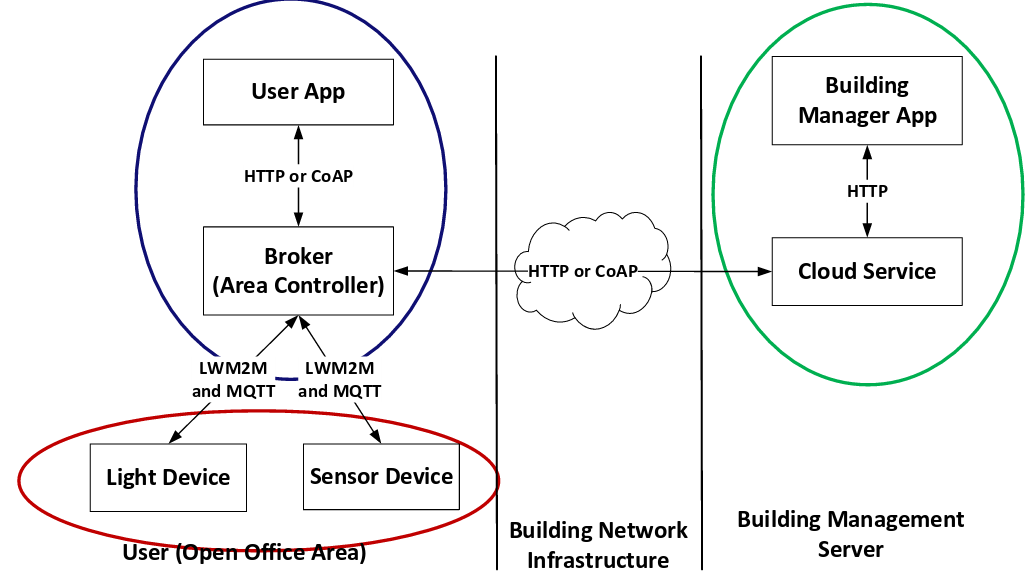
\includegraphics[width=1\linewidth]{img/design}
		\caption{This Figure is from the lecture slides on IoT \cite{slides}}
		\label{fig:fig1}
	\end{center}
\end{figure}


\section{Implementation, Architecture and Protocols}

There are four significant deliverables for the broker group. Each of them had to be dealt with separately: 
\begin{enumerate}
	\item There is a user app for the user to control the light/s, which was selected to be a Android app for this showcase.
	\item mDNS discovery service. Avahi was chosen for this job and is built into linux or can be used with python for integration into a python project.
	\item LWM2M (Rest API) - a 'light weight machine to machine communication' with end device as well as maintaining a CoAP/HTTP server. Leshan was chosen for this task and is written in Java.
	\item MQTT broker which allows lights and sensors to communicate basic commands between one and other with this well suited subscribe and publish service. Mosquitto version 1.4.8 was used for this and installed on linux.
\end{enumerate}

\textit{A laptop with Ubuntu 16.04 64-bit was used to run all these modules except the Android app which was run with an emulator and designed on a Windows computer.}

Documentation was found in the thorough tutorial library provided on the course website \cite{tut}. The architecture is somewhat predefined but many design options were left up to the teams. All communication and information will pass through the broker on its way to the endpoint.

\begin{figure}[h]
	\begin{center}
		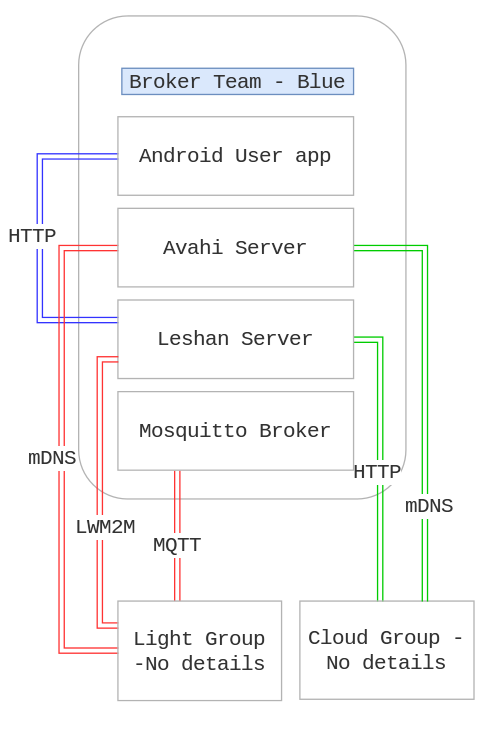
\includegraphics[width=0.6\linewidth]{img/overview}
		\caption{}
		\label{fig:fig2}
	\end{center}
\end{figure}

\section{Questionnaire and work-flow}

Here are some generic 
\begin{enumerate}
	
	\item Why did you choose that implementation setup.
	\begin{itemize}
		\item The implementation setup shown in Figure \ref{fig:fig2} was chosen for the project. The reason is completely based on the knowledge base of the group and team. This was done to try to shorten the development time. A joint opinion was made towards using HTTP between cloud and broker and Leshan for main communication between end device and broker. The android user app was chosen because it is also written in Java like Leshan it would help to keep to as few programming languages as possible. There was little to no choice regarding MQTT broker (Mosquitto) nor the mDNS service (Linux built in).
	\end{itemize}
	\item How long did it take to learn to use the LWM2M framework, Leshan.
	\begin{itemize}
		\item This was one of the larges obstacles where neither of the group members and done much work in Java. The learning curve is reasonable were already familiar with object orientated programming. Thus it took around a 3 days, netto, to create a base for the project and then soma additional hours adapting to the other groups architecture. 
	\end{itemize}
	\item Go long did it take to implement your part of the system.
	\begin{itemize}
		\item The whole process started early but the time spent on the project increased when getting closer to the plugfest. In total the work took 5 days per person, assuming approximately 10 hours a day.
	\end{itemize}
	\item what were the steps you go through for implementing your part of the system.
	\begin{itemize}
		\item Firstly research about the whole project and then further research on each of the communication methods and protocols. Which operating system to pick for the broker, linux. Then piece by piece the parts were done individually until completed enough to puzzle together with the other teams.
	\end{itemize}
	\item What were the difficulties that you encounter during implementation.
	\begin{itemize}
		\item Mostly, there were problems using Leshan and making it work so that it could be developed in Visual studio (Windows only) and then run on the linux machine. It is possible to develop on linux in Eclipse, but that is a terrible idea were Visual studio is much further developed for high level use. Solution was to use git for the whole Leshan project and only build with Linux after pulling the latest updates. This was the main difficulty but other smaller ones will be mentioned later.
	\end{itemize}
	\item What were the notable programming limitations of the chosen tools, libraries or frameworks.
	\begin{itemize}
		\item Not really. They are high level and well documented.
	\end{itemize}
	\item  What are your suggestion as a programmer for better experience in implementing IoT application. 
	\begin{itemize}
		\item Just to try to create one central location where all the team members can meet and easily connect to the same network, with internet access preferably. This seems maybe a small advice, but this is very important. And if possible to have all devices powered on at all times with ssh access such that people can work on them from anywhere. The cloud and broker team could also use their raspberry pis to develop the project and would not have to meet as often and allow for more debugging every now and then.
	\end{itemize}

\end{enumerate}

\subsection{LWM2M: CoAP and HTTP with Leshan}


LWM2M is the fundamental ingredient in the broker. It provides a REST API for both CoAP and HTTP which can both be modified to serve the needs of the system. Leshan operates with a server/client infrastructure. Thus the broker runs a server module and other devices connecting to it use a client module. The android app and the cloud service take advantage of the HTTP protocol and the end-device uses the CoAP protocol.


\subsection{User app: Android}

\subsection{mDNS: Avahi broker}
mDNS stands for Multicast Domain Name System and it can inform other devices on the same network of the IP of the host. It uses the same structure as DNS but it is a zero configuration service. Avahi implements this zero configuration network discovery profile. On linux Avahi is already installed an requires no extra installation. Both the cloud and end device need to take advantage of this service and can retrieve the IP address with discovery, thus then connecting to the remaining system such a MQTT or Leshan. Figure \ref{fig:avahi} shows how this can be done.

\begin{figure}[h]
	\begin{center}
		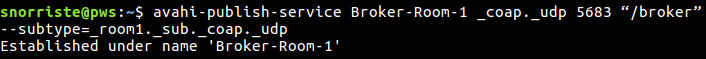
\includegraphics[width=1.1\linewidth]{img/avahi}
		\caption{The bash command for running the avahi client on linux}
		\label{fig:avahi}
	\end{center}
\end{figure}


For embedding this into Java, Python or any other high level programming language, it is possible to call the bash command with a 'OS' library and read the output. Setting this up on the broker only required running on startup. Problems during the development were mostly related to port and firewall issues with the laptop or network connection.

\subsection{MQTT: Mosquitto}
MQTT stands for MQ Telemetry Transport and is a very light weight publish and subscribe protocol. The Mosquitto broker is installed on the linux machine and then the clients can both publish messages to topics and subscribe to the topics as well. This module worked seamlessly after install. In the testing section it can be observed how messages are published (this is only for making sure from the broker side that the MQTT broker is working). Figure \ref{fig:mqtt2} shows the Mosquitto messaging broker installed on the linux computer.

\begin{figure}[h]
	\begin{center}
		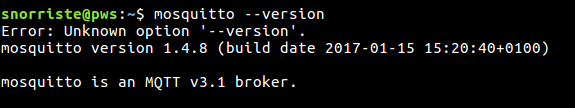
\includegraphics[width=.8\linewidth]{img/mqtt2}
		\caption{Mosquitto install on the linux machine}
		\label{fig:mqtt2}
	\end{center}
\end{figure}

\section{Product Testing}

From day one all code had to be tested frequently and thoroughly, eliminating errors and all bad test cases. Most testing had to be done with the Leshan server. A dummy client was created to simulated the end device and then HTTP request where sent from browser and tested with the android app as well.

\subsection{MQTT testing}

Testing was done on MQTT for making sure that clients could connect to it and communicate the FREE/OCCUPIED between the sensor and light device. That part worked for all teams connecting to the system. As can be seen in Figure \ref{fig:mqtt3}.
\begin{figure}[h]
	\begin{center}
		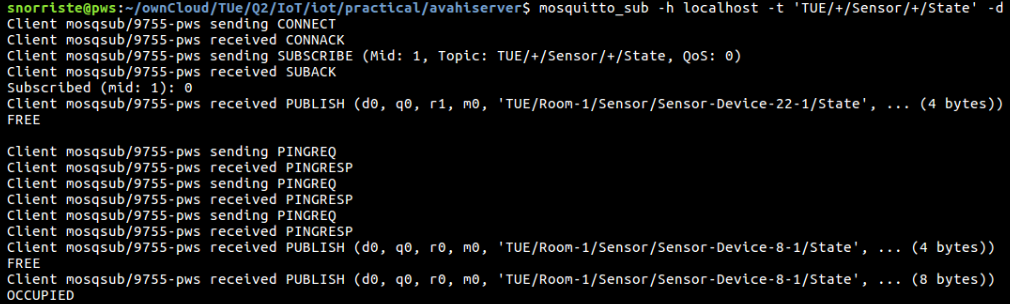
\includegraphics[width=\linewidth]{img/mqtt3}
		\caption{Mosquitto tested during Plugfest with other teams. MQTT broker works and clients can communicate.}
		\label{fig:mqtt3}
	\end{center}
\end{figure}

\subsection{Leshan Testing}

This section will show testing of Leshan, how it responded to requests and how the development interface looks like. In Figure \ref{fig:observe} the log for the Leshan server is displayed when an request from the web app is made to observe a sensor value (resource 10350).

\begin{figure}[h]
	\begin{center}
		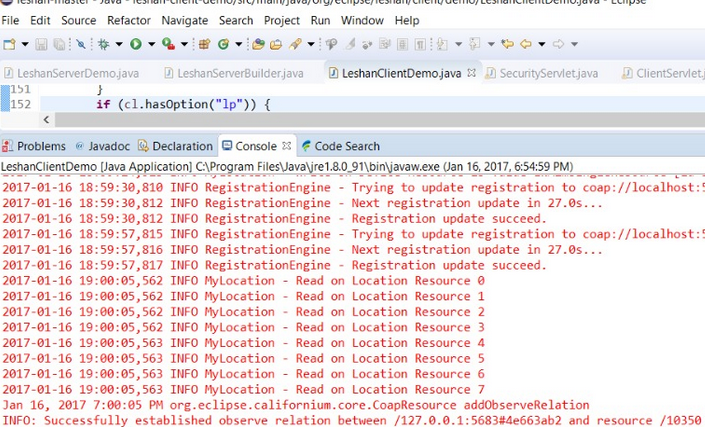
\includegraphics[width=\linewidth]{img/screenshot-observe}
		\caption{It can be seen here that an observation was made on an resource}
		\label{fig:observe}
	\end{center}
\end{figure}

An important part to be working is the updating of ownership and thus it is useful to show the testing of the part. In Figure \ref{fig:own} the Leshan server log can be seen when the Cloud group updates the ownership via their manager web app seen in Figure \ref{fig:cloudown}.

\begin{figure}[h]
	\begin{center}
		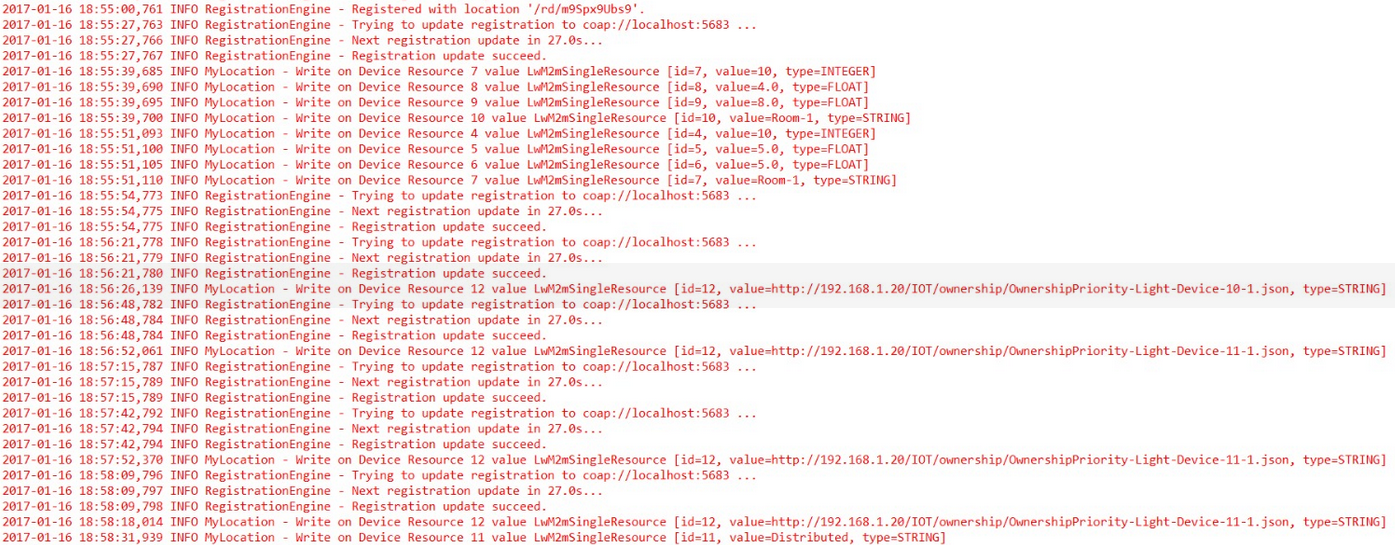
\includegraphics[width=1.18\linewidth]{img/screenshot-ownership}
		\caption{Here it can be seen that the ownership was updated from another IP address, namely the Cloud}
		\label{fig:own}
	\end{center}
\end{figure}

\begin{figure}[h]
	\begin{center}
		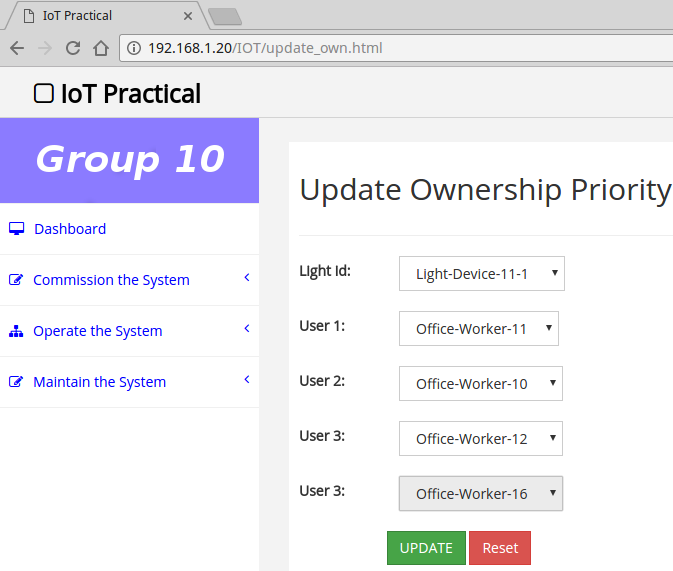
\includegraphics[width=.8\linewidth]{img/screenshot-cloud-ownership}
		\caption{The Cloud group updates the ownership in the Leshan server via their web app in this picture. The IP matching the IP in the logs in Figure \ref{fig:own}}
		\label{fig:cloudown}
	\end{center}
\end{figure}

\subsection{App Testing}
In Figure \ref{fig:app} the app can be seen working with multiple clients. The light can be controlled as indicated.

\subsection{Avahi Testing}

Avahi was tested multiple times with the red team. Figure \ref{fig:avahi} shows the command publish the service and then if the client uses the same parameters it will connect. 
\section{Discussion and results}
\section{Evaluation}

Now the systems has been developed so that it can talk to any end-device with the predefined information sharing. The broker can be turned on, make it self discoverable to any end-device (mDNS), allow for communication between light and sensor device (MQTT) and finally allows for end-devices to register as clients in Leshan and be accessed by the cloud with jetty inside Leshan. This is the complete, simplified, architecture use case.	
\section{Reflection}


\section{Contribution}
\subsection{UserApp(Android)}
begin{enumerate}
\item LoginActivity: Validating the entered user details against server- Snorri.
\item ClientActivity: Collecting information related to current state of the system from broker- SaiKrishna.
\item ControlActivity: Creating User interface for light objects-Snorri
\item  ControlActivity: Communicating the updated light state to the broker- Sai Krishna.
\item Utilities:Creating and handling HTTP requests,parsing JSON information from server-Sai Krishna.
end{enumerate}

\subsection{Server(Leshan)}
begin{enumerate}
\item ClientServlet:Handling read, write and observation requests from cloud and UserApp-Snorri
\item EventServlet:Performing operations during registrations, creating new observation requests- Sai Krishna

\item EventServlet(CentralizedDeployment):Handling new observations,updating databases,centralized Deployment routine-Snorri

\item Security Servlet:Storing User details received from cloud and handling Login validation requests from UserAPP- Sai Krishna.

\item Utilities:Json parsing,Dummy Clients for testing-Sai Krishna

\subsection{Avahi}-Creating network discovery for both clients and cloud service-Snorri.
\subsection{MQTT}-Creatig MQTT broker client publish and subscriptions -Snorri.

\subsection{Report} Report for the project-Snorri and Sai Krishna.

\pagebreak

\section{Appendix A - Large Screenshots}

\begin{figure}[h]
	\begin{center}
		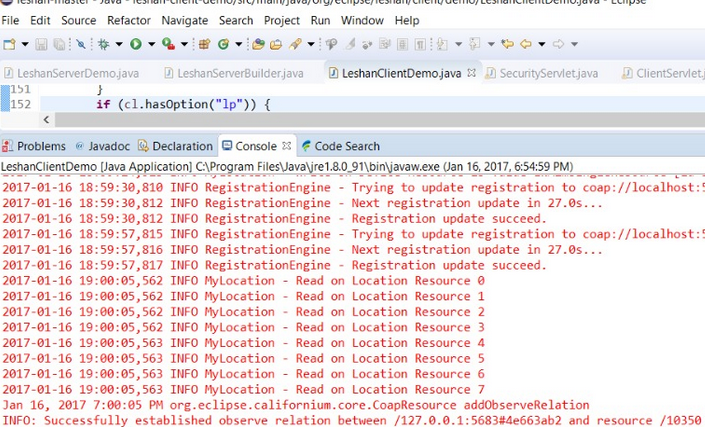
\includegraphics[width=\linewidth]{img/screenshot-observe}
		\caption{It can be seen here that an observation was made on an resource}
		\label{fig:observe}
	\end{center}
\end{figure}

\begin{figure}[h!]
	\begin{center}
		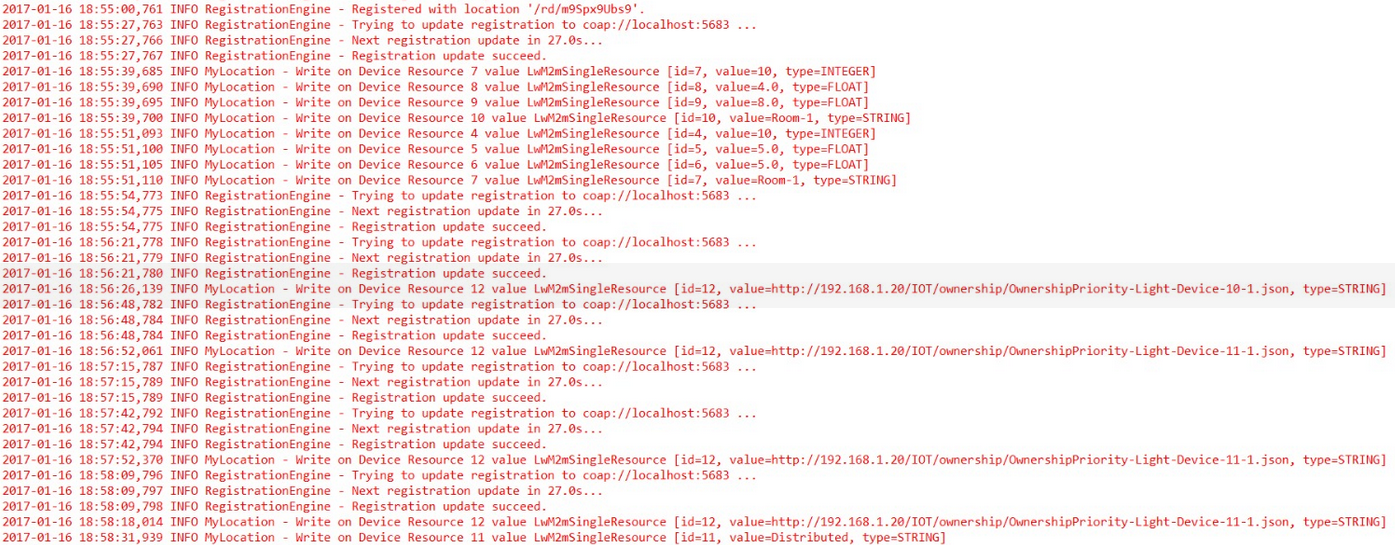
\includegraphics[width=1.18\linewidth]{img/screenshot-ownership}
		\caption{Here it can be seen that the ownership was updated from another IP address, namely the Cloud}
		\label{fig:own}
	\end{center}
\end{figure}

\begin{figure}[h!]
	\begin{center}
		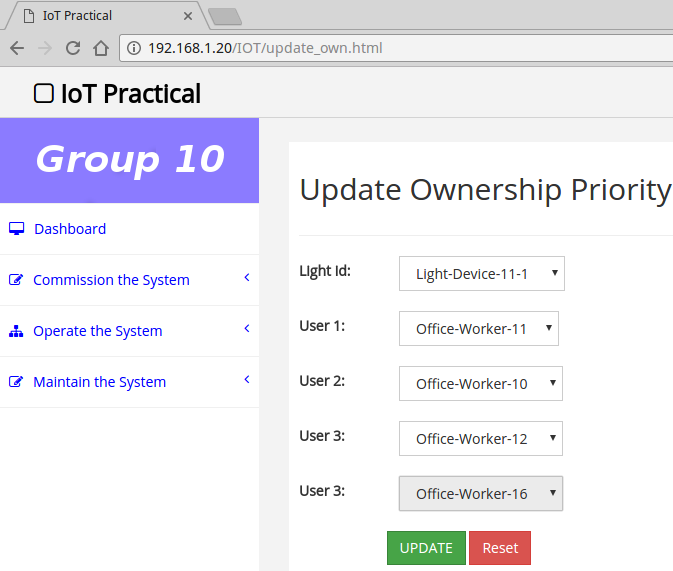
\includegraphics[width=.6\linewidth]{img/screenshot-cloud-ownership}
		\caption{The Cloud group updates the ownership in the Leshan server via their web app in this picture. The IP matching the IP in the logs in Figure \ref{fig:own}}
		\label{fig:cloudown}
	\end{center}
\end{figure}

\begin{figure}[h!]
	\begin{center}
		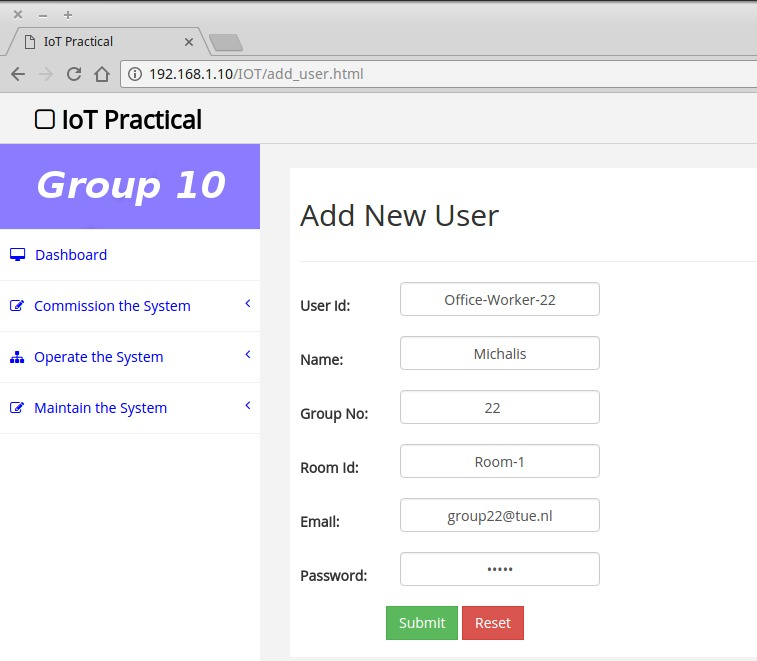
\includegraphics[width=.6\linewidth]{img/newUserCloud}
		\caption{A new user added seen from the Cloud's web application}
		\label{fig:newuser}
	\end{center}
\end{figure}
\begin{figure}[h!]
	\begin{center}
		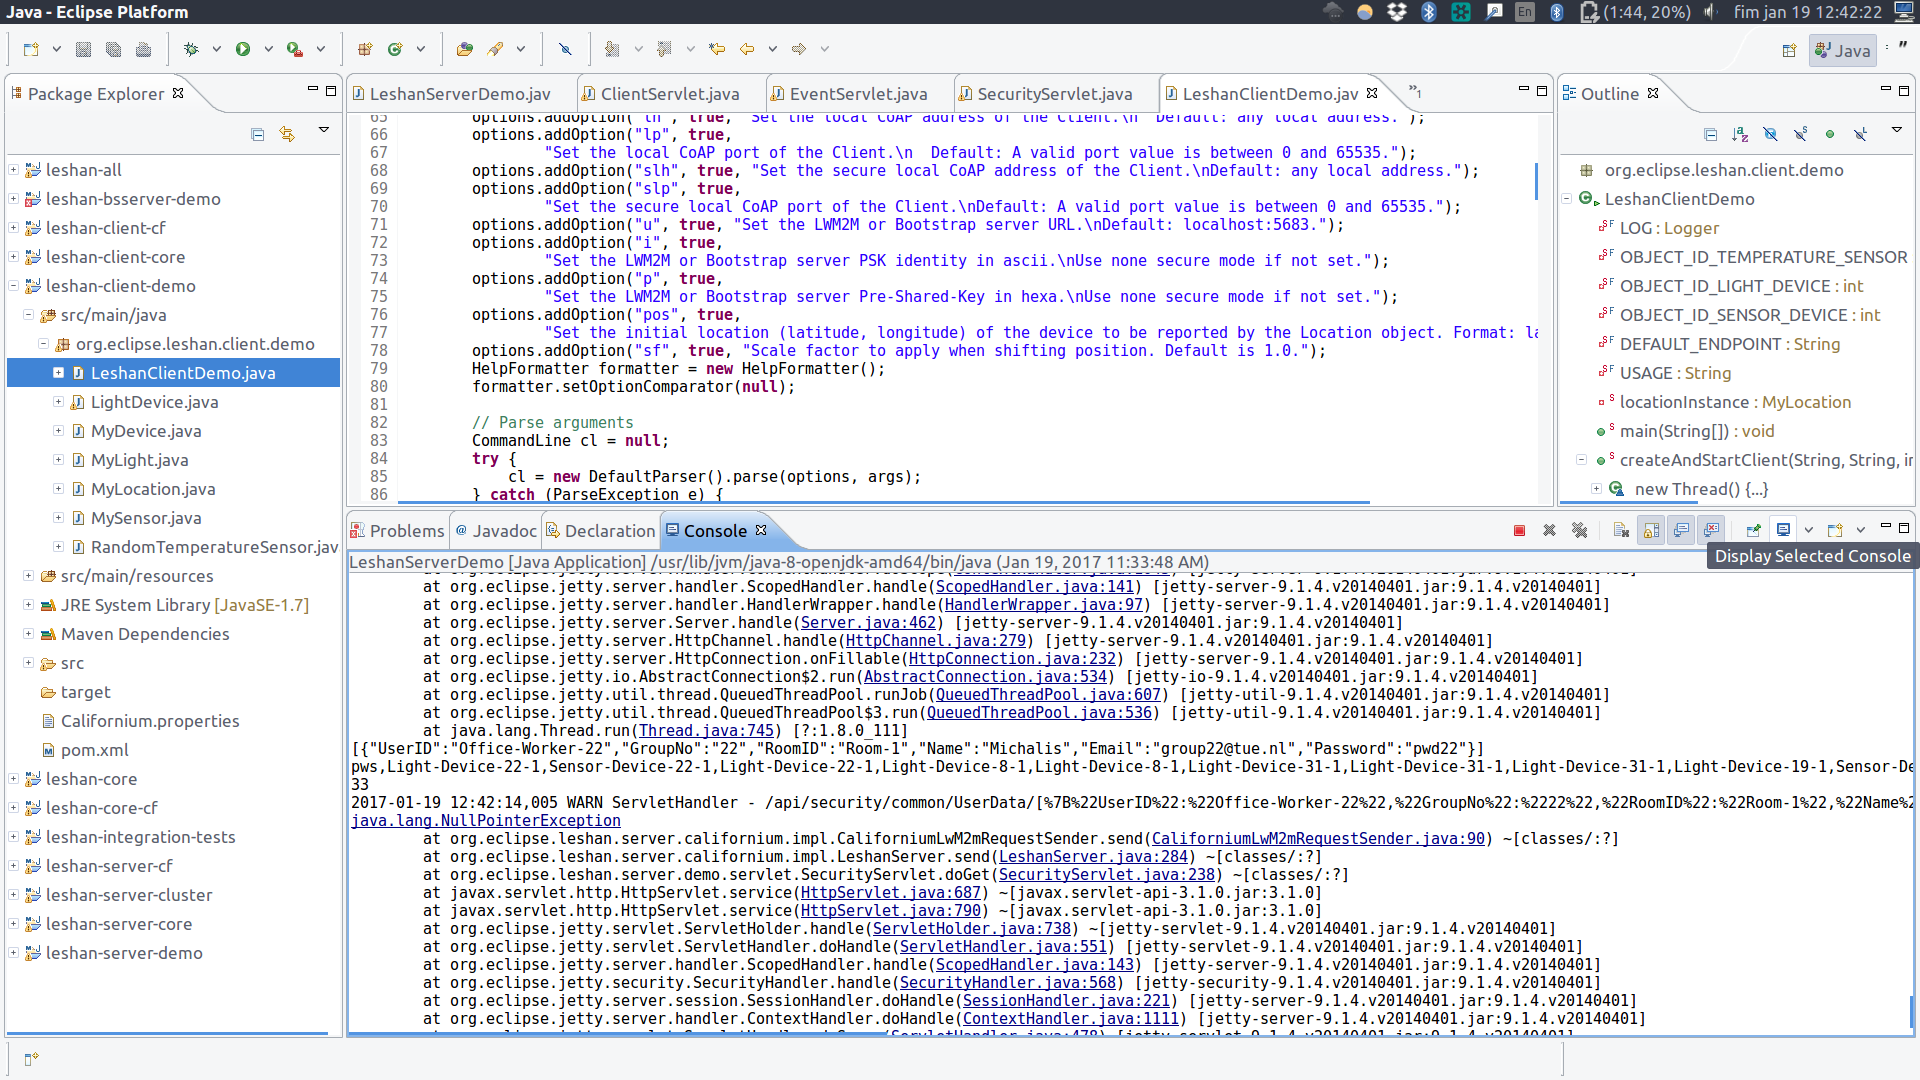
\includegraphics[width=\linewidth]{img/newUser}
		\caption{A new user add seen from the leshan server which can now be used to log into the app to control the light}
		\label{fig:newusercloud}
	\end{center}
\end{figure}

\newpage
\printbibliography

\end{document}